	\begin{frame}
		\Huge{\centerline{Execution of}}
		\Huge{\centerline{Multi-Agent Systems}}
	\end{frame}
	
	%------------------------------------------------
	
	\begin{frame}
		\frametitle{Semantics of Computational Run }
		\begin{block}{Definition}
			The execution of a 2APL multi-agent system with initial configuration $A_1,...,A_n, \chi$ is the set of computation runs $CR(A_1,...,A_n, \chi)$ of the 2APL transition system.
		\end{block}
		\begin{block}{Definition}
			A computation run $CR(s0)$ is a sequence $s_0,...$ where $s_i$ is a
			configuration, and $ \forall{i>0} : s_{i−1} \rightarrow s_i$ is a transition in the transition system.
		\end{block}
		
	\end{frame}
	
	
	%------------------------------------------------
	
	\begin{frame}
		\frametitle{Single-Agent Deliberation Cycle}
		\begin{figure}
			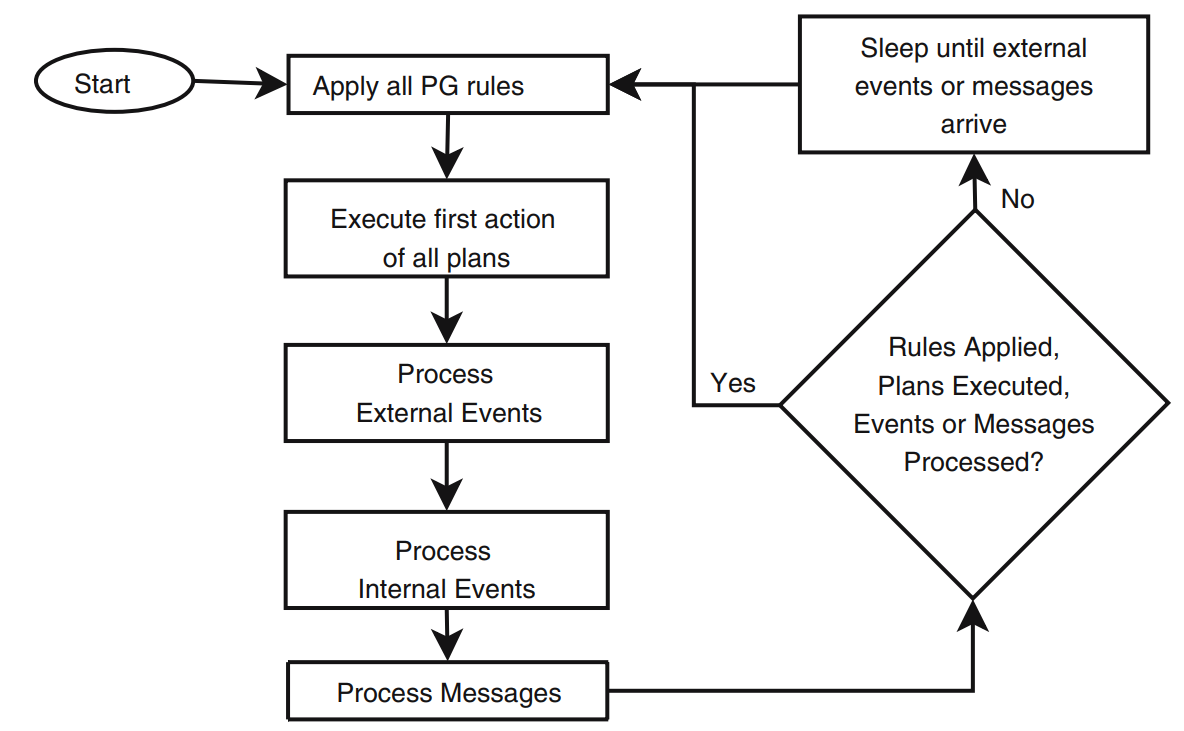
\includegraphics[width=1\textwidth]{deliberation-cycle-individual-2apl}
		\end{figure}
	\end{frame}
	
	%------------------------------------------------
	
	\begin{frame}
		\frametitle{Characteristics of the Deliberation Cycle (I)}
		\begin{itemize}
			
			\item The interpreter of 2APL executes individual agents and the environment in
			parallel in an interleaving mode.\\~\\
			
			\item Each cycle starts by applying all applicable PG-rules, each rule only one time. \\~\\
			
			\item The DC proceeds by executing only the first actions of all plans. In order to allow all plans to get a chance to be executed. \\~\\
			
			\item  Internal and external events and messages are processed by applying the first applicable PC-rule. \\~\\
			
		\end{itemize}
	\end{frame}
	
	\begin{frame}
		\frametitle{Characteristics of the Deliberation Cycle (II)}
		\begin{itemize}
			
			\item If the execution of a plan fails, then the plan will either be repaired in the same
			deliberation cycle or get re-executed in the next deliberation cycle. \\~\\
			
			\item If the first action of a failed plan is a belief update, test, adopt
			goal, abstract or external action and there is no plan repair rule to
			repair it, then the failed plan may be successfully executed in the next deliberation cycle. \\~\\
			
		\end{itemize}
	\end{frame}